\documentclass[a4paper, 10pt]{article}
\usepackage[utf8]{inputenc}
\usepackage[danish]{babel}
\usepackage{verbatim}
\usepackage{amsmath}
\usepackage{listings}
\usepackage{graphicx}

\title{Fundations of Computer Graphics\\ Ugeopgave 3}
\author{Mads Ohm Larsen}

\begin{document}
\lstset{language=C, basicstyle=\footnotesize, numbers=left, stepnumber=2, numberstyle=\tiny, frameround=tttt, frame=tlBR, captionpos=b}
\maketitle

% Introduktion, the why?
\section{Introduktion}
I denne uge vil vi gerne tegne trekanter.
Trekanterne skal helst være fyldte trekanter.
Grunden til at vi er så vilde med trekanter, er at alle polygoner kan brydes ned til trekanter, det vil sige de kan blive trianguleret.
Det betyder at vi kan tegne alle former og figurer ved hjælp af trekanter, og derfor behøver vi ikke kunne tegne andet, da, hvis vi for eksempel, gerne vil have en firkant, bare kan tegne to trekanter.

Når vi tegner trekanter vil vi følge en vis konvention, nemlig at højre- og topkanter ikke bliver tegnet.
Dette gøres simpelthen fordi at så står pixelsne ikke og flimre mellem to forskellige farver, hvis vi tegner to trekanter ved siden af hinanden i forskellige farver.
Det betyder selvfølgelig at alle trekanter bliver en lille smule mindre end de burde være, men de bliver tilgengæld også det pænere at kigge på.


%%%%%%%%%%%%%%%%%%%%%%%%%%%%%%%%%%%%%%%%
% Kanter og hvad fanden er en trekant? %
%%%%%%%%%%%%%%%%%%%%%%%%%%%%%%%%%%%%%%%%
\section{TreKANTER}
Hvad er det præcis en trekant er?
En trekant er en figur, med tre kanter.
Skal vi tegne den, kan vi altså tegne de tre kanter og alle pixels inden i denne konvekse figur.
Vi skal dog have i bagtankerne at vi ikke skal tegne højre- og topkanter.

Den nemmeste måde at tegne trekanter på, er således ved at tegne såkaldte skanlinier.
Med skanlinier menes en vandret linie, som skær både venstre- og højrekanterne.
Dette kan selvfølgelig gøres \textit{dumt} ved faktisk at beregne skæringerne i flydende tal og derefter afrundet resultatet.

Vi vil, ligesom vores line rasterizer fra sidste uge, lave en inkrementiel algoritme til at tegne disse trekanter.
Det betyder imidlertid at vi først må vide hvordan en kant ser ud, vi laver altså en \texttt{edge\_rasterizer} først, og med denne kan vi lave en \texttt{triangle\_rasterizer}.

%%%%%%%%%%
% KANTER %
%%%%%%%%%%
\section{Kanter}

%%%%%%%%%%%%%%%%%%%%
% HVAD ER EN KANT? %
%%%%%%%%%%%%%%%%%%%%
\subsection{Hvad er en kant?}
En meget kort beskrivelse af en kant er en linie, fra $(x_{start}, y_{start})$ til $(x_{stop}, y_{stop})$.

Det er sådan man normalt kender kanter i en f.eks. en trekant, men vi vil gerne lidt mere.
Vi vil gerne kunne sige at flere linie stykker danner en kant.
Vi tænker derfor ikke på en kant, som en faktisk kant i en f.eks. en trekant, men derimod som et sæt af liniestykker, som går fra et punkt til et andet, eventuelt gennem et eller flere midterpunkter.

Hvor om alting er, så kigger vi kun på de kanter som består af et liniestykke, da vi kan kæde disse sammen på en smart måde, som jeg vil komme ind på senere.
En kant kan beskrives som en linie med følgende ligning:

\begin{equation}
y = \frac{dy}{dx} x + \beta \nonumber 
\end{equation}

som vi allerede kender så godt fra vores line rasterizer. Dette er selvfølgelig blot den normale ligning for en linie, hvor $dy$ er ændring i $y$ og $dx$ er ændring i $x$.
Da vi skankonvertere langs y-aksen, skriver vi denne ligning om til

\begin{align}
x &= \frac{dx}{dy} (y - \beta) \nonumber\\
  &= \frac{dx}{dy} y - \frac{dx}{dy} \beta \nonumber
\end{align}

En ændring på x-aksen, vil således være 

\begin{equation}
( x_{i+1} - x_i ) = \frac{dx}{dy} ( y_{i+1} - y_i ) \nonumber
\end{equation}

Denne kan igen skrives om til

\begin{align}
x_{i+1} &= x_i + \frac{dx}{dy} ( y_{i+1} - y_i ) \nonumber\\
        &= x_i + \frac{dx}{dy} \Delta y \nonumber
\end{align}

Da vi gerne vil regne pixels, kan vi antage at $\Delta y = 1$, og vi får da at i en given skanlinie $(y_{i+p})$ er den tilhørende x-værdi: 

\begin{align}
x_{i+p} &= x_i + \sum^p_{j=1} \frac{dx}{dy} \nonumber\\
        &= x_i + \frac{\sum^p_{j=1}dx}{dy}
\end{align}

Vi har såldes delt vores værdi op i en heltals og en brøk del.
Hvis brøken giver mere end $1$ skal vi tælle vores heltal det antal ned (vi starter med at lave kanter med negativ hældning), ellers skal vi ikke bruge brøken til noget.
Brøken er kun større end $1$ hvis tælleren er større end nævneren, så derfor kan vi lave en sammenligning i stedet for en division og en sammenligning.

Når vi laver kanter med positiv hælding, skal vi sørger for at komme på den rigtige side af stregen, og vi skal derfor starte én gang længere inde.
Dette vil jeg ikke komme mere ind på i denne korte gennemgang af hvordan vi tegner kanter.

%%%%%%%%%%%%%%
% ALGORITMEN %
%%%%%%%%%%%%%%
\subsection{Algoritmen}
Når vi implemtere algoritmen, kan vi, i stedet for at regne hele summen fra (\ref{sumformel}), blot holde styr på den pågældende iteration.

Har vi en funktion \texttt{set\_dot(x, y)}, som tegner en pixel i $(x,y)$, kan vi gøre følgende for at tegne alle pixels på en linie

\begin{lstlisting}
int dx          = x_stop - x_start;
int x_step      = ( dx < 0 ) ? -1 : 1;
int numerator   = |dx|;
int denominator = y_stop - y_start;
int accumulator = ( dx > 0 ) ? denominator : 1;
int x           = x_start;

for( int y = y_start; y < y_stop; ++y ) {
    set_dot( x, y );
    accumulator += numerator;
    while( accumulator > denominator ) {
        x           += x_step;
        accumulator -= denominator;
    }
}
\end{lstlisting}

%%%%%%%%%%%%%%%
% TREKANTERNE %
%%%%%%%%%%%%%%%
\section{Trekanterne}
Der findes fire generiske trekanter.
To har horisontale kanter, top henholdsvis bund kanten.
De to andre har en lige kant fra det nederste venstre hjørne til det øverste venstre hjørne.
De andre to kanter i disse to kan vi sætte sammen til én kant, som jeg kort var inde på tidligere.
Vi kan sætte dem sammen, da vi er sikre på at de mødes i et hjørne (ellers ville det jo ikke være en kant i en trekant) og vi er sikre på at den øverste af disse ender i det øverste venstre hjørne.
Det vil heller ikke påvirke skanlinierne af samme grund, og det er derfor en smart ting at gøre.

Når vi har begge kanter på plads, er det ingen problem at tegne en trekant.
Her skal vi jo blot tegne alle punkterne i en skanlinie, bortset fra dem der ligger på en top- eller højrekant.

Vores algoritme er således rimelig simpel:

\begin{enumerate}
\item Lav en venstre \texttt{edge\_rasterizer} (\texttt{left})
\item Lav en højre \texttt{edge\_rasterizer} (\texttt{right})
\item Få koordinaterne $(x_l, y_l) = (\texttt{left.x()}, \texttt{left.y()})$
\item Få koordinaterne $(x_r, y_r) = (\texttt{right.x()}, \texttt{right.y()})$
\item Hvis der er punkter på skanlinien, altså hvis $\left\lbrace (x_l, y_l) \dots (x_r - 1, y_r) \right\rbrace \not = \emptyset$, tegn disse pixels
\item Lad de to \texttt{edge\_rasterizer}s gå et skridt op af deres kant
\item Hvis der stadig er flere \texttt{fragments} tilbage, gå til 3, ellers returnere falsk
\end{enumerate}

Vi skal altså blot vide hvordan vi klarer disse skridt og så kan vi tegne vores trekanter.
De to første siger næsten sig selv, og dog, da vi lige skal finde ud af hvilken en der skal have to linier, som kant.
Her må vi kigge på de fire typer jeg beskrev før.
De to første, med vandrette kanter, er nemme nok, her kan vi simpelthen blot smide hele den kant væk, og kun bruge de to andre.
Vi skal dog huske at den nederste kant stadig skal tegnes.

Med de to andre er det lidt sværere.
Her skal vi finde ud af om det er højre eller venstre side, som har to linier.
Først må vi finde ud af hvordan vi skal navngive punkterne i disse kanter.
Hvis vi kalder dem \texttt{lower\_left}, \texttt{upper\_left} henholdsvis \texttt{the\_other} og lader som om de er 3-dimensionele vektore, med z-værdi lig nul, kan vi tage krydsproduktet af de to linier, som bliver udspændt af \texttt{lower\_left} og \texttt{upper\_left} henholdsvis \texttt{lower\_left} og \texttt{the\_other}, og derved finde ud af hvilken type trekant de er.
Hvis krydsproduktet er $0$ betyder det at de to kanter er co-linær, og det er altså ikke en trekant vi har fat i, men derimod blot et liniestykke.
Er krydsproduktet negativt betyder det, at det er den venstre kant, som er to linier og sidst, hvis krydsproduktet er positivt, betyder det at det er den højre kant, som er to linier.

Nu er det altså blot at tegne alle pixels mellem de to \texttt{edge\_rasterizer}s, og så er trekanten tegnet.

\subsection{Lidt kode at slutte af på}
Til sidst vil jeg blot vise resultatet, i form af billeder, samt en lille stumpkode, navnligt \texttt{next\_fragment()} og en hjælpefunktion, \texttt{SearchForNonEmptyScanline()}, som bruges til at finde den næste skanline, som indeholde pixels, som skal tegnes.

Først \texttt{next\_fragment()}
\begin{lstlisting}
void next_fragment()    
{
    if( this->valid && 
        this->left.more_fragments() && 
        this->right.more_fragments() ) {
	
       if( this->y_current > this->left.y() && 
            this->y_current > this->right.y() ) {
	    
            this->valid = false;
	} else if( this->x_current >= this->right.x() - 1 ) {
	    
            if( !this->SearchForNonEmptyScanline() ) {
		this->valid = false;
	    }
	
        } else {
	    this->x_current += 1;
	}
    } else {
	this->valid = false; 
    }
}
\end{lstlisting} 

Her løber vi alle de pixels igennem, som skal tegnes, en af gangen.
Jeg gør her brug af min hjælpefunktion \texttt{SearchForNonEmptyScanline()}, som ser således ud
\pagebreak
\begin{lstlisting}
bool SearchForNonEmptyScanline()
{
    do {
	this->left.next_fragment();
	this->right.next_fragment();

	if( this->left.more_fragments() && 
            this->right.more_fragments() ) {
	    
            this->x_current = this->left.x();
	    this->y_current = this->left.y();
	} else {
	    break;
	}
    } while( this->x_current > this->right.x() - 1 );

    return this->valid && 
           this->left.more_fragments() && 
           this->right.more_fragments();
}
\end{lstlisting}

Denne returnere sand, hvis den finder en ikke-tom skanline, samt sætter x- og y-koordinater for den pixel, som er længst til venstre på denne skanline.

Kører man \texttt{framework} og trykker \texttt{T} nogle gange, kommer man frem til følgende figurer, som også er vedlagt denne rapport i en større størrelse:

\begin{center}
\centering
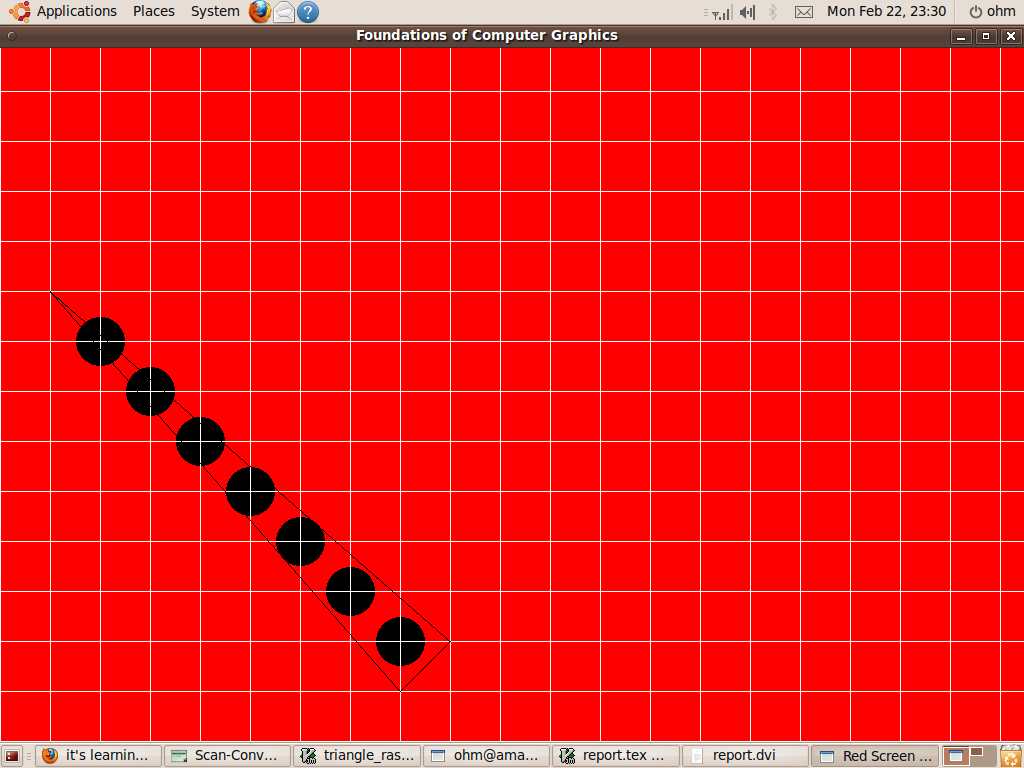
\includegraphics[width=0.99\textwidth]{triangle1.eps}
\end{center}

\begin{center}
\centering
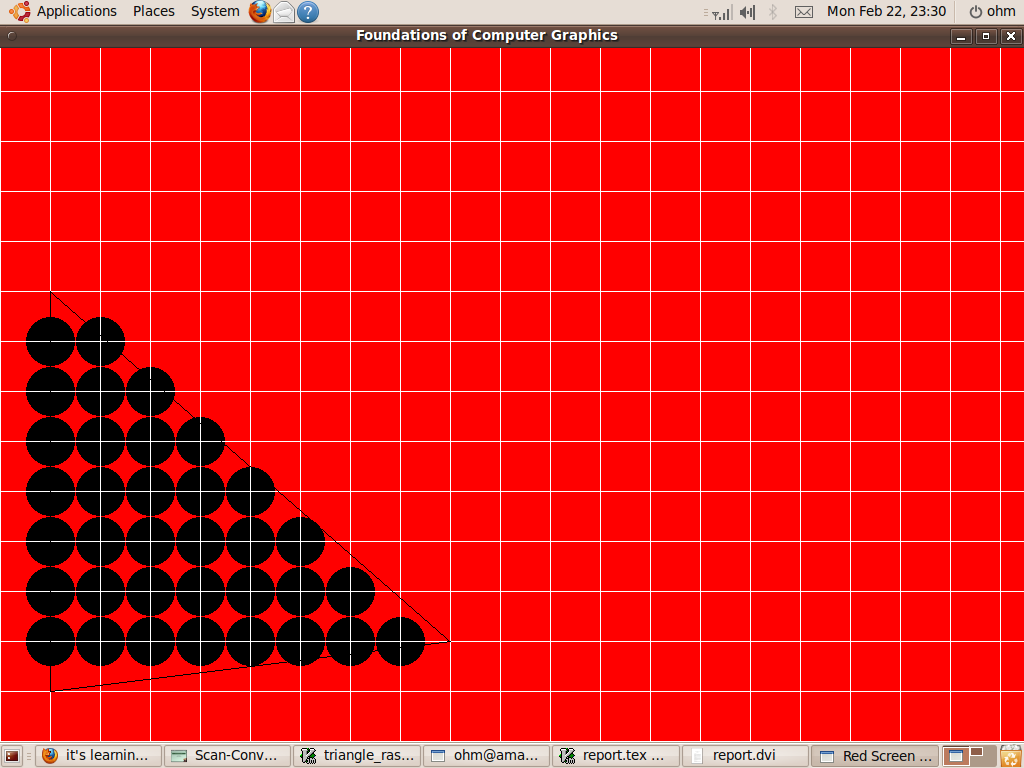
\includegraphics[width=0.99\textwidth]{triangle2.eps}
\end{center}

\begin{center}
\centering
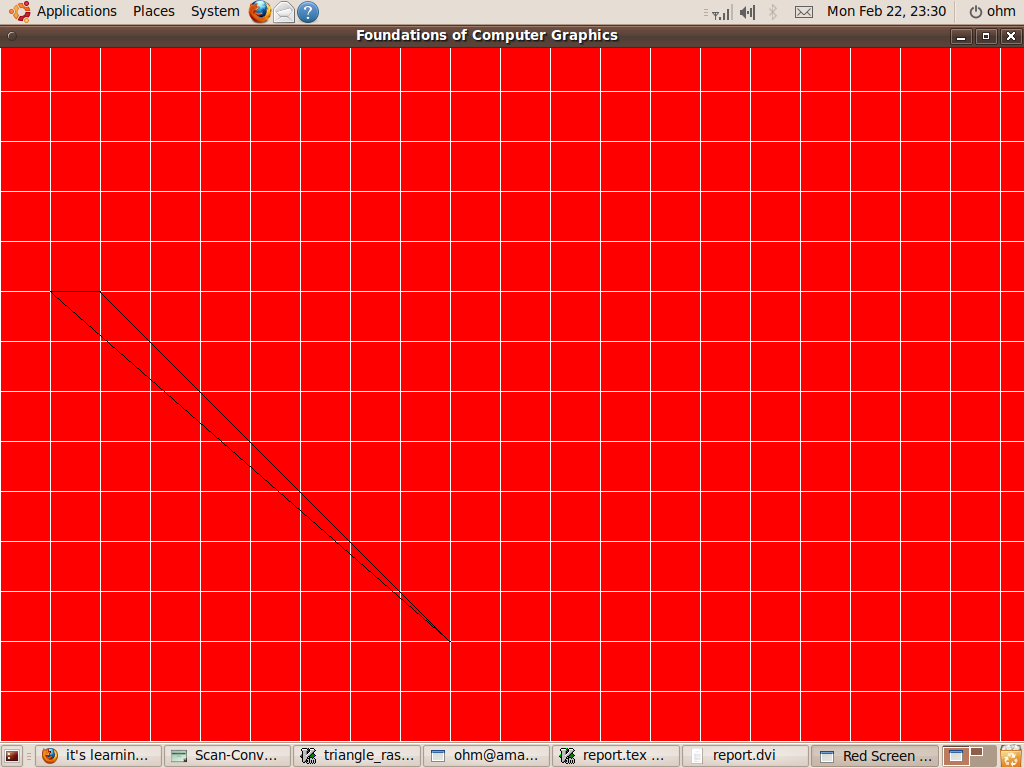
\includegraphics[width=0.99\textwidth]{triangle3.eps}
\end{center}



\end{document}
